\documentclass{article}
\usepackage{amsmath, amssymb, graphicx, tikz, pgfplots, booktabs, xcolor}
\pgfplotsset{compat=1.18}

\newenvironment{lesson-meta}{}{}
\newenvironment{item-analysis}{}{}
\newenvironment{model-discuss}{}{}
\newenvironment{concept-box}{}{}
\newenvironment{concept-summary}{}{}
\newenvironment{example}[1]{}{}
\newenvironment{tryit}[1]{}{}
\newenvironment{practice}[2]{}{}
\newenvironment{te-addendum}[2]{}{}
\newcommand{\answer}[1]{}
\newcommand{\placeholder}[2]{}
\newcommand{\uncertain}[2]{#1}
\newcommand{\te}[1]{}

\begin{document}

\begin{lesson-meta}
\textbf{6-3 Logarithms}
\textbf{I CAN...} evaluate and simplify logarithms.

\textbf{VOCABULARY}
\begin{itemize}
    \item common logarithm
    \item logarithm
    \item logarithmic function
    \item natural logarithm
\end{itemize}

\textbf{ESSENTIAL QUESTION} What are logarithms and how are they evaluated?
\end{lesson-meta}

\begin{model-discuss}
\textbf{CRITIQUE \& EXPLAIN}

Earthquakes make seismic waves through the ground. The equation $y = 10^x$ relates the height, or amplitude, in microns on a seismograph, of a seismic wave, $y$, and the power, or magnitude, $x$, of the ground-shaking it can cause.

Taylor and Chen used different methods to find the magnitude of the earthquake with amplitude 5,500.

\begin{tabular}{|c|c|}
\hline
\textbf{Magnitude, $x$} & \textbf{Amplitude, $y$} \\
\hline
2 & 100 \\
3 & 1,000 \\
? & 5,500 \\
4 & 10,000 \\
\hline
\end{tabular}

\vspace{1em}
\noindent
\textbf{Taylor}\\
5,500 is halfway between 1,000 and 10,000.\\
3.5 is halfway between 3 and 4.\\
The magnitude is about 3.5.

\vspace{1em}
\noindent
\textbf{Chen}\\
$y = 10^x$\\
$10^3 = 1,000$\\
$10^4 = 10,000$\\
$10^{3.5} \approx 3,162$\\
$10^{3.7} \approx 5,012$\\
$10^{3.8} \approx 6,310$\\
$10^{3.74} \approx 5,500$\\
The magnitude is about 3.74.

\vspace{1em}
\textbf{A.} What is the magnitude of an earthquake with amplitude 100,000? How do you know?

\textbf{B. Construct Arguments} Critique Taylor's and Chen's work. Is each method valid? Could either method be improved?

\textbf{C.} Describe how to express the exact value of the desired magnitude.
\end{model-discuss}

\begin{example}{1}
\textbf{Understand Logarithms}

Solve $2^x = 8$.

The operation in $2^x = 8$ is exponentiation. To solve this equation, you need an inverse operation that answers the question, ``To what exponent would you raise the base 2 to get 8?''

\textbf{USE STRUCTURE}
Creating the notation $\log_2 x$ to represent the exponent to which you raise 2 to get $x$ is similar to creating the radical notation $\sqrt{x}$ to represent one number you can square to get $x$.

\placeholder{diagram}{Callout: Division is the inverse of multiplication, so you can divide both sides by 2 to solve the equation. $2x = 8 \rightarrow \frac{2x}{2} = \frac{8}{2} \rightarrow x = 4$}

A \textit{logarithm} is the inverse of exponentiation.
To solve the equation $2^x = 8$, you can write $\log_2 8 = x$. Solving this gives $\log_2 8 = 3$ because $2^3 = 8$.

\placeholder{diagram}{Callout pointing to $\log_2 8$: This is read ``logarithm base 2 of 8'' or ``log base 2 of 8.''}

The \textbf{logarithm} base $b$ of $x$ is defined as follows.
$\log_b x = y$ if and only if $b^y = x$, for $b > 0$, $b \neq 1$, and $x > 0$.

The \textbf{logarithmic function} $y = \log_b x$ is the inverse of the exponential function $y = b^x$.
\end{example}

\begin{tryit}{1}
Write the logarithmic form of $y = 8^x$.
\end{tryit}

\begin{concept-box}
\textbf{CONCEPT Exponential and Logarithmic Forms}

\textbf{Exponential form} shows that a \textcolor{red}{base} raised to an \textcolor{green}{exponent} equals the \textcolor{purple}{result}.
$$a^b = c$$

\textbf{Logarithmic form} shows that the log of the \textcolor{purple}{result} with the given \textcolor{red}{base} equals the \textcolor{green}{exponent}.
$$\log_a c = b$$

\placeholder{diagram}{Callout pointing to $c$: When written in logarithmic form, the number that was the result of the exponential equation is often called the argument.}

\textbf{STUDY TIP}
A fact family for 2, 3, and 5 are the four addition and subtraction equations that relate the three numbers. Think of exponential and logarithmic forms as a fact family for the three numbers given.
\end{concept-box}

\begin{example}{2}
\textbf{Convert Between Exponential and Logarithmic Forms}

\textbf{A. What is the logarithmic form of $3^4 = 81$?}

The \textcolor{red}{base} is \textcolor{red}{3}, the \textcolor{green}{exponent} is \textcolor{green}{4}, and the \textcolor{purple}{result} is \textcolor{purple}{81}.

So, in logarithmic form,
$$3^4 = 81 \rightarrow \log_3 81 = 4.$$
The logarithmic form of $3^4 = 81$ is $\log_3 81 = 4$.

\textbf{B. What is the exponential form of $\log_{10} 1,000 = 3$?}

The base is 10, the exponent is 3, and the result (or argument) is 1,000.

So, in exponential form,
$$\log_{10} 1,000 = 3 \rightarrow 10^3 = 1,000.$$
The exponential form of $\log_{10} 1,000 = 3$ is $10^3 = 1,000$.
\end{example}

\begin{tryit}{2}
\textbf{a.} What is the logarithmic form of $7^3 = 343$?

\textbf{b.} What is the exponential form of $\log_4 16 = 2$?
\end{tryit}

\begin{example}{3}
\textbf{Evaluate Logarithms}

\textbf{GENERALIZE}
The output of any exponential function of the form $y = b^x$, with $b > 0$, is always a positive number. Therefore, the input of a logarithmic function must also be a positive number. Why?

What is the value of each logarithmic expression?

\textbf{A. $\log_5 125$}
THINK: $5^? = 125$
Since $5^3 = 125$, $\log_5 125 = 3$.

\textbf{B. $\log_{\frac{1}{4}} 16$}
THINK: $\left(\frac{1}{4}\right)^? = 16$
Since $\left(\frac{1}{4}\right)^{-2} = 16$, $\log_{\frac{1}{4}} 16 = -2$.

\textbf{C. $\log_3 0$}
THINK: $3^? = 0$
There is no such power, so $\log_3 0$ is undefined.

\textbf{D. $\log_2 2^8$}
THINK: $2^? = 2^8$
Since $2^8 = 2^8$, $\log_2 2^8 = 8$.
\end{example}

\begin{tryit}{3}
What is the value of each logarithmic expression?

\textbf{a.} $\log_3\left(\frac{1}{81}\right)$ \qquad \textbf{b.} $\log_7(-7)$ \qquad \textbf{c.} $\log_5 5^9$
\end{tryit}

\begin{concept-box}
\textbf{CONCEPT Common Logarithms and Natural Logarithms}

The base 10 logarithm is called the \textbf{common logarithm} and is written as $\log x$ with the base of 10 implied.

The base $e$ logarithm is called the \textbf{natural logarithm} and is written as $\ln x$.
\end{concept-box}

\begin{example}{4}
\textbf{Evaluate Common and Natural Logarithms}

\textbf{STUDY TIP}
Scientific calculators have keys for the common logarithm (LOG) and the natural logarithm (LN).

What is the value of each logarithmic expression to the nearest ten-thousandth?

\placeholder{diagram}{Callout: Evaluate the exponential forms to reinforce these inverse operations.}

\textbf{A. $\log 900$}
$\log 900 \approx 2.9542$ $\rightarrow$ $10^{2.9542} \approx 900$

\textbf{B. $\ln e$}
$\ln e = 1$ $\rightarrow$ $e^1 = e$

\textbf{C. $\ln (-1.87)$}
$\ln (-1.87) \rightarrow \text{ERROR}$ $\rightarrow$ $e^? = -1.87$
There is no exponent to which $e$ can be raised in order to get a negative number, so $\ln (-1.87)$ is undefined.

\placeholder{illustration}{Calculator screen showing: \newline log(900) \newline 2.954242509 \newline ln(e) \newline 1 \newline ln(-1.87) \newline Error}
\end{example}

\begin{tryit}{4}
What is the value of each logarithmic expression to the nearest ten-thousandth?

\textbf{a.} $\log 321$ \qquad \textbf{b.} $\ln 1,215$ \qquad \textbf{c.} $\log 0.17$
\end{tryit}

\begin{example}{5}
\textbf{Solve Equations With Logarithms}

\textbf{COMMON ERROR}
Remember that 10 is not a coefficient, but a base. You cannot divide both sides by 10 and then add 1 to solve for $x$.

What is the solution to each equation? Round to the nearest thousandth.

\textbf{A.} $25 = 10^{x-1}$
\begin{align*}
25 &= 10^{x-1} \\
\log 25 &= x - 1 \quad \text{(\placeholder{diagram}{Callout: Convert to logarithmic form.}})\\
1 + \log 25 &= x \\
2.398 &\approx x
\end{align*}

\textbf{B.} $\ln (2x + 3) = 4$
\begin{align*}
\ln (2x + 3) &= 4 \\
2x + 3 &= e^4 \quad \text{(\placeholder{diagram}{Callout: Convert to exponential form.}})\\
2x + 3 &\approx 54.598 \\
2x &\approx 51.598 \\
x &\approx 25.799
\end{align*}
\end{example}

\begin{tryit}{5}
Solve each equation. Round to the nearest thousandth.

\textbf{a.} $\log (3x - 2) = 2$ \qquad \textbf{b.} $e^{x+2} = 8$
\end{tryit}

\begin{example}{6}
\textbf{Use Logarithms to Solve Problems}

The seismic energy, $x$, in joules can be estimated based on the magnitude, $m$, of an earthquake by the formula $x = 10^{1.5m+12}$. What is the magnitude of an earthquake with a seismic energy of $4.2 \times 10^{20}$ joules?

\placeholder{illustration}{Earthquake Magnitude Scale showing categories: 2.5 or less, 2.5 to 5.4, 5.5 to 6.0, 6.1 to 6.9, 7.0 to 7.9, 8.0 or greater, next to a drawing of a cracked landscape.}

\textbf{Formulate} \quad Substitute $4.2 \times 10^{20}$ for $x$ in the formula.
$$4.2 \times 10^{20} = 10^{1.5m+12}$$

\textbf{Compute} \quad Solve the equation for $m$.
\begin{align*}
4.2 \times 10^{20} &= 10^{1.5m+12} \\
\log (4.2 \times 10^{20}) &= 1.5m + 12 \quad \text{(\placeholder{diagram}{Callout: Rewrite in logarithmic form.}})\\
20.6 &\approx 1.5m + 12 \\
5.75 &\approx m
\end{align*}

\textbf{Interpret} \quad The magnitude of the earthquake is about 5.75.
Verify the answer: $10^{1.5(5.75)+12} \approx 4.2 \times 10^{20}$
\end{example}

\begin{tryit}{6}
What is the magnitude of an earthquake with a seismic energy of $1.8 \times 10^{23}$ joules?
\end{tryit}

\begin{concept-summary}
\textbf{CONCEPT SUMMARY Logarithms}

\begin{tabular}{p{0.2\textwidth}p{0.3\textwidth}cp{0.3\textwidth}}
& \textbf{Exponential Form} & & \textbf{Logarithmic Form} \\
\textbf{ALGEBRA} & $b^x = y$ & $\leftrightarrow$ & $\log_b y = x$ \\
\textbf{WORDS} & The base raised to the exponent is equal to a result. & & The logarithm with a base $b$ of the result (or argument) is equal to the exponent. \\
\textbf{NUMBERS} & $3^4 = 81$ & $\leftrightarrow$ & $\log_3 81 = 4$ \\
\end{tabular}
\end{concept-summary}

\section*{PRACTICE \& PROBLEM SOLVING}

\subsection*{Do You UNDERSTAND?}

\begin{practice}{1}{?}
\textbf{ESSENTIAL QUESTION} What are logarithms and how are they evaluated?
\end{practice}

\begin{practice}{2}{?}
\textbf{Error Analysis} Amir said the expression $\log_5 (-25)$ simplifies to $-2$. Explain Amir's possible error.
\end{practice}

\begin{practice}{3}{?}
\textbf{Vocabulary} Explain the difference between the common logarithm and the natural logarithm.
\end{practice}

\begin{practice}{4}{?}
\textbf{Make Sense and Persevere} How can logarithms help to solve an equation such as $10^t = 656$?
\end{practice}

\subsection*{Do You KNOW HOW?}

Write each equation in logarithmic form.
\begin{practice}{5}{?}
$2^{-6} = \frac{1}{64}$
\end{practice}

\begin{practice}{6}{?}
$e^4 \approx 54.6$
\end{practice}

Write each equation in exponential form.
\begin{practice}{7}{?}
$\log 200 \approx 2.301$
\end{practice}

\begin{practice}{8}{?}
$\ln 25 \approx 3.22$
\end{practice}

Evaluate the expression.
\begin{practice}{9}{?}
$\log_4 64$
\end{practice}

\begin{practice}{10}{?}
$\log \frac{1}{100}$
\end{practice}

\begin{practice}{11}{?}
$\ln e^5$
\end{practice}

\begin{practice}{12}{?}
Solve for $x$. $4e^x = 7$.
\end{practice}

\subsection*{UNDERSTAND}

\begin{practice}{13}{?}
\textbf{Make Sense and Persevere} If the LN button on your calculator were broken, how could you still use your calculator to find the value of the expression $\ln 65$?
\end{practice}

\begin{practice}{14}{?}
\textbf{Error Analysis} Describe and correct the error a student made in solving an exponential equation.

\begin{align*}
16e^t &= 98 \\
e^t &= 6.125 \\
6.125t &= \ln e \quad \text{\textcolor{red}{\textbf{X}}} \\
t &= \frac{\ln e}{6.125}
\end{align*}
\end{practice}

\begin{practice}{15}{?}
\textbf{Higher Order Thinking} Use the graph of $y = 3^x$ to estimate the value of $\log_3 50$. Explain your reasoning.

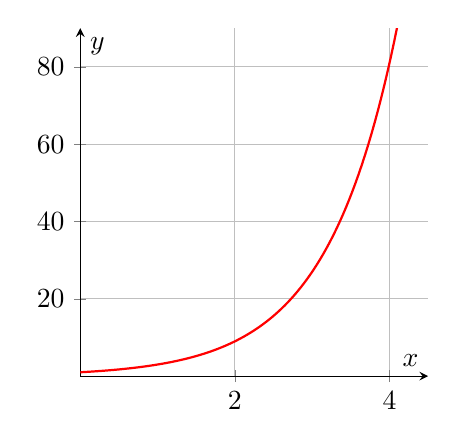
\begin{tikzpicture}
\begin{axis}[
    width=6cm, height=6cm,
    xmin=0, xmax=4.5,
    ymin=0, ymax=90,
    axis lines=middle,
    xlabel={$x$},
    ylabel={$y$},
    xtick={0,2,4},
    ytick={20,40,60,80},
    domain=0:4.1,
    samples=100,
    grid=both
]
\addplot[red, thick] {3^x};
\end{axis}
\end{tikzpicture}
\end{practice}

\begin{practice}{16}{?}
\textbf{Generalize} For what values of $x$ is the expression $\log_4 x < 0$ true?
\end{practice}

\begin{practice}{17}{?}
\textbf{Use Structure} A student says that $\log_3\left(\frac{1}{27}\right)$ simplifies to $-3$. Is the student correct? Explain.
\end{practice}

\begin{practice}{18}{?}
\textbf{Use Structure} Explain why the expression $\ln 1,000$ is not equal to 3.
\end{practice}

\begin{practice}{19}{?}
\textbf{Construct Arguments} Explain why $\log_b b^x = x$. Explain why $e^{\ln x} = x$.
\end{practice}

\subsection*{PRACTICE}

Write the logarithmic form of each exponential equation. SEE EXAMPLE 1
\begin{practice}{20}{?}
$y = 4^x$
\end{practice}

\begin{practice}{21}{?}
$y = 10^x$
\end{practice}

\begin{practice}{22}{?}
$y = 7^x$
\end{practice}

\begin{practice}{23}{?}
$y = a^x$
\end{practice}

Write each equation in logarithmic form. SEE EXAMPLE 2
\begin{practice}{24}{?}
$3^8 = 6,561$
\end{practice}

\begin{practice}{25}{?}
$e^{-3} \approx 0.0498$
\end{practice}

\begin{practice}{26}{?}
$5^0 = 1$
\end{practice}

\begin{practice}{27}{?}
$7^3 = 343$
\end{practice}

Write each equation in exponential form. SEE EXAMPLE 2
\begin{practice}{28}{?}
$\log \frac{1}{100} = -2$
\end{practice}

\begin{practice}{29}{?}
$\log_8 64 = 2$
\end{practice}

\begin{practice}{30}{?}
$\ln 148.41 \approx 5$
\end{practice}

\begin{practice}{31}{?}
$\log_2 \frac{1}{32} = -5$
\end{practice}

Evaluate each logarithmic expression. SEE EXAMPLE 3
\begin{practice}{32}{?}
$\log_5 \frac{1}{125}$
\end{practice}

\begin{practice}{33}{?}
$\log_6 (-216)$
\end{practice}

\begin{practice}{34}{?}
$\log_3 3^4$
\end{practice}

\begin{practice}{35}{?}
$\log_2 32$
\end{practice}

\begin{practice}{36}{?}
$\log_9 729$
\end{practice}

\begin{practice}{37}{?}
$\log_8 \frac{1}{64}$
\end{practice}

\begin{practice}{38}{?}
$\log_7 0$
\end{practice}

\begin{practice}{39}{?}
$\log_7 7^a$
\end{practice}

Use a calculator to evaluate each expression. Round to the nearest ten-thousandth. SEE EXAMPLE 4
\begin{practice}{40}{?}
$\log 78.5$
\end{practice}

\begin{practice}{41}{?}
$\log 0.24$
\end{practice}

\begin{practice}{42}{?}
$\ln (-37)$
\end{practice}

\begin{practice}{43}{?}
$\ln 41.5$
\end{practice}

\begin{practice}{44}{?}
$\log 12$
\end{practice}

\begin{practice}{45}{?}
$\ln 3$
\end{practice}

Solve each equation. Round answers to the nearest ten-thousandth. SEE EXAMPLES 5 AND 6
\begin{practice}{46}{?}
$\log (7x + 6) = 3$
\end{practice}

\begin{practice}{47}{?}
$2.75e^t = 38.6$
\end{practice}

\begin{practice}{48}{?}
$\ln (3x - 1) = 2$
\end{practice}

\begin{practice}{49}{?}
$10^{t+1} = 50$
\end{practice}

\begin{practice}{50}{?}
$1.5e^t = 27$
\end{practice}

\begin{practice}{51}{?}
$\log (x - 3) = -1$
\end{practice}

\begin{practice}{52}{?}
How long does it take for \$250 to grow to \$600 at 4\% annual percentage rate compounded continuously? Round to the nearest year.
\end{practice}

\subsection*{APPLY}

\begin{practice}{53}{?}
\textbf{Model with Mathematics} Michael invests \$1,000 in an account that earns a 4.75\% annual percentage rate compounded continuously. Peter invests \$1,200 in an account that earns a 4.25\% annual percentage rate compounded continuously. Which person's account will grow to \$1,800 first?
\end{practice}

\begin{practice}{54}{?}
\textbf{Reason} The Richter magnitude of an earthquake is $R = 0.67\log(0.37E) + 1.46$, where $E$ is the energy (in kilowatt-hours) released by the earthquake.

\textbf{a.} What is the magnitude of an earthquake that releases 11,800,000,000 kilowatt-hours of energy? Round to the nearest tenth.

\textbf{b.} How many kilowatt-hours of energy would an earthquake have to release in order to be an 8.2 on the Richter scale? Round to the nearest whole number.

\textbf{c.} What number of kilowatt-hours of energy would an earthquake have to release in order for walls to crack? Round to the nearest whole number.

\placeholder{illustration}{Image showing a cracked wall with the text: "At a richter magnitude of 4 and above, the walls in your house may start to crack." Below is a scale from 1 to 10 with "Not felt" on the left and "Extreme" on the right. The number 4 is circled.}
\end{practice}

\begin{practice}{55}{?}
\textbf{Reason} The function $c(t) = 108e^{-0.08t} + 75$ calculates the temperature, in degrees Fahrenheit, of a cup of coffee that was handed out a drive-thru window $t$ minutes ago.

\textbf{a.} What is the temperature of the coffee in the instant that it is handed out the window?

\textbf{b.} After how many minutes is the coffee in the cup 98 degrees Fahrenheit? Round to the nearest whole minute.
\end{practice}

\subsection*{ASSESSMENT PRACTICE}

\begin{practice}{56}{?}
Sheba invests \$500 in an account that earns 2.5\% annual percentage rate compounded continuously. How long will it take for her account to grow to \$700?
\end{practice}

\begin{practice}{57}{?}
\textbf{SAT/ACT} In the equation $\log_3 a = b$, if $b$ is a whole number, which of the following CANNOT be a value for $a$?

\textbf{A} 1 \qquad \textbf{B} 3 \qquad \textbf{C} 6 \qquad \textbf{D} 9 \qquad \textbf{E} 81
\end{practice}

\begin{practice}{58}{?}
\textbf{Performance Task} Money is deposited into two separate accounts. The money in one account is compounded continuously. The money in the other account is not compounded continuously. Neither account has any money withdrawn in the first 6 years.

\begin{tabular}{|c|c|c|}
\hline
\textbf{Year} & \textbf{Account 1 Balance (\$)} & \textbf{Account 2 Balance (\$)} \\
\hline
0 & 400 & 500 \\
1 & 433.31 & 575 \\
2 & 469.40 & 650 \\
3 & 508.50 & 725 \\
4 & 550.85 & 800 \\
5 & 596.72 & 875 \\
\hline
\end{tabular}

\textbf{Part A} Write a function to calculate the amount of money in each account given $t$, the number of years since the account was opened. Describe the growth in each account.

\textbf{Part B} Will the amount of money in Account 1 ever exceed the amount of money in Account 2? Explain. If so, when will that occur?
\end{practice}

\end{document}